\documentclass[11pt]{article}
\usepackage[a4paper, margin=1in]{geometry}
\usepackage{amsmath, amssymb}
\usepackage{graphicx}
\usepackage{xcolor}
\usepackage{tikz}
\usetikzlibrary{positioning,shapes}
\usepackage{pgfplots}
\usepackage{amsthm}
\newtheorem{theorem}{Theorem}
\pgfplotsset{compat=1.18}
\usepackage{booktabs}
\usepackage{tabularx}
\usepackage{multirow}
\usepackage{fancyhdr}
\usepackage{hyperref}
\usepackage{lipsum}
\usepackage{listings}
\usepackage{enumitem}

\lstset{
  basicstyle=\ttfamily\small,
  keywordstyle=\color{blue},
  commentstyle=\color{green!60!black},
  stringstyle=\color{red},
  numbers=left,
  numberstyle=\tiny\color{gray},
  frame=single,
  breaklines=true,
}

\pagestyle{fancy}
\fancyhf{}
\fancyhead[L]{SyncTeX Comprehensive Test}
\fancyhead[R]{\thepage}

\title{A Comprehensive Document for SyncTeX Testing}
\author{Bookokrat Test Suite}
\date{April 2026}

\begin{document}

\maketitle
\tableofcontents
\newpage

% ============================================================================
% SECTION 1: Introduction and prose
% ============================================================================
\section{Introduction}

This document is designed to exercise the SyncTeX synchronization engine across
a wide variety of LaTeX content types. It spans approximately 20 pages and
includes plain text, mathematical formulas, code listings, tables, figures,
TikZ diagrams, and mixed-content pages.

\subsection{Motivation}

When building a PDF viewer with SyncTeX support, it is critical to verify that
forward search (source line to PDF position) and inverse search (PDF position to
source line) work correctly across all content types. A document containing only
plain text is insufficient because:

\begin{itemize}
  \item Mathematical formulas generate different synctex node structures than text.
  \item Tables and figures create floating environments with complex positioning.
  \item Code listings generate verbatim content with line-by-line correspondence.
  \item TikZ graphics produce embedded drawing commands that interact with the
        synctex coordinate system in non-trivial ways.
\end{itemize}

\subsection{Document Structure}

The remainder of this document is organized as follows:
\begin{enumerate}
  \item Section~\ref{sec:calculus} covers differential and integral calculus.
  \item Section~\ref{sec:linalg} covers linear algebra and matrix operations.
  \item Section~\ref{sec:stats} covers probability and statistics.
  \item Section~\ref{sec:graphs} contains TikZ diagrams and pgfplots charts.
  \item Section~\ref{sec:code} includes source code listings.
  \item Section~\ref{sec:tables} demonstrates complex table layouts.
  \item Section~\ref{sec:mixed} combines all content types on single pages.
  \item Section~\ref{sec:prose} contains extended prose passages.
\end{enumerate}

\lipsum[1-2]

\newpage

% ============================================================================
% SECTION 2: Calculus
% ============================================================================
\section{Differential and Integral Calculus}
\label{sec:calculus}

\subsection{Limits and Continuity}

The formal definition of a limit states that for every $\varepsilon > 0$
there exists a $\delta > 0$ such that:

\begin{equation}
  0 < |x - a| < \delta \implies |f(x) - L| < \varepsilon
  \label{eq:limit}
\end{equation}

A function $f$ is continuous at a point $a$ if
$\lim_{x \to a} f(x) = f(a)$.

\subsection{Derivatives}

The derivative of $f$ at $x$ is defined as:

\begin{equation}
  f'(x) = \lim_{h \to 0} \frac{f(x+h) - f(x)}{h}
  \label{eq:derivative}
\end{equation}

Common derivative rules include:

\begin{align}
  \frac{d}{dx}[x^n] &= nx^{n-1} \label{eq:power} \\
  \frac{d}{dx}[e^x] &= e^x \label{eq:exp} \\
  \frac{d}{dx}[\sin x] &= \cos x \label{eq:sin} \\
  \frac{d}{dx}[\cos x] &= -\sin x \label{eq:cos} \\
  \frac{d}{dx}[\ln x] &= \frac{1}{x} \label{eq:ln}
\end{align}

The chain rule for composite functions:
\begin{equation}
  \frac{d}{dx}[f(g(x))] = f'(g(x)) \cdot g'(x)
  \label{eq:chain}
\end{equation}

\subsection{Integration}

The fundamental theorem of calculus connects differentiation and integration:

\begin{theorem}[Fundamental Theorem of Calculus]
If $f$ is continuous on $[a,b]$ and $F$ is an antiderivative of $f$ on $[a,b]$, then:
\begin{equation}
  \int_a^b f(x)\,dx = F(b) - F(a)
  \label{eq:ftc}
\end{equation}
\end{theorem}

Important integral formulas:

\begin{align}
  \int x^n\,dx &= \frac{x^{n+1}}{n+1} + C, \quad n \neq -1 \\
  \int e^x\,dx &= e^x + C \\
  \int \frac{1}{x}\,dx &= \ln|x| + C \\
  \int \sin x\,dx &= -\cos x + C \\
  \int \cos x\,dx &= \sin x + C
\end{align}

\subsection{Taylor Series}

Exactly Super Not The Taylor series expansion of $f(x)$ around $a$:
\begin{equation}
  f(x) = \sum_{n=0}^{\infty} \frac{f^{(n)}(a)}{n!}(x-a)^n
  \label{eq:taylor}
\end{equation}

Notable expansions:
\begin{align}
  e^x &= \sum_{n=0}^{\infty} \frac{x^n}{n!} = 1 + x + \frac{x^2}{2!} + \frac{x^3}{3!} + \cdots \\
  \sin x &= \sum_{n=0}^{\infty} \frac{(-1)^n x^{2n+1}}{(2n+1)!} = x - \frac{x^3}{3!} + \frac{x^5}{5!} - \cdots \\
  \cos x &= \sum_{n=0}^{\infty} \frac{(-1)^n x^{2n}}{(2n)!} = 1 - \frac{x^2}{2!} + \frac{x^4}{4!} - \cdots \\
  \frac{1}{1-x} &= \sum_{n=0}^{\infty} x^n = 1 + x + x^2 + x^3 + \cdots, \quad |x| < 1
\end{align}

\lipsum[3]

\newpage

% ============================================================================
% SECTION 3: Linear Algebra
% ============================================================================
\section{Linear Algebra and Matrix Operations}
\label{sec:linalg}

\subsection{Matrix Definitions}

A matrix $A \in \mathbb{R}^{m \times n}$ is a rectangular array of real numbers:
\begin{equation}
  A = \begin{pmatrix}
    a_{11} & a_{12} & \cdots & a_{1n} \\
    a_{21} & a_{22} & \cdots & a_{2n} \\
    \vdots & \vdots & \ddots & \vdots \\
    a_{m1} & a_{m2} & \cdots & a_{mn}
  \end{pmatrix}
  \label{eq:matrix}
\end{equation}

\subsection{Determinants}

For a $2 \times 2$ matrix:
\begin{equation}
  \det \begin{pmatrix} a & b \\ c & d \end{pmatrix} = ad - bc
\end{equation}

For a $3 \times 3$ matrix, using cofactor expansion along the first row:
\begin{equation}
  \det \begin{pmatrix}
    a_{11} & a_{12} & a_{13} \\
    a_{21} & a_{22} & a_{23} \\
    a_{31} & a_{32} & a_{33}
  \end{pmatrix}
  = a_{11}(a_{22}a_{33} - a_{23}a_{32})
  - a_{12}(a_{21}a_{33} - a_{23}a_{31})
  + a_{13}(a_{21}a_{32} - a_{22}a_{31})
\end{equation}

\subsection{Eigenvalues and Eigenvectors}

Given a square matrix $A$, an eigenvector $\mathbf{v}$ and eigenvalue $\lambda$ satisfy:
\begin{equation}
  A\mathbf{v} = \lambda\mathbf{v}
  \label{eq:eigen}
\end{equation}

The eigenvalues are found by solving the characteristic equation:
\begin{equation}
  \det(A - \lambda I) = 0
  \label{eq:characteristic}
\end{equation}

\subsection{Singular Value Decomposition}

Any matrix $A \in \mathbb{R}^{m \times n}$ can be decomposed as:
\begin{equation}
  A = U \Sigma V^T
  \label{eq:svd}
\end{equation}
where $U \in \mathbb{R}^{m \times m}$ and $V \in \mathbb{R}^{n \times n}$ are orthogonal matrices,
and $\Sigma \in \mathbb{R}^{m \times n}$ is a diagonal matrix of singular values.

\lipsum[4-5]

\newpage

% ============================================================================
% SECTION 4: Probability and Statistics
% ============================================================================
\section{Probability and Statistics}
\label{sec:stats}

\subsection{Probability Distributions}

The probability density function of the normal distribution:
\begin{equation}
  f(x) = \frac{1}{\sigma\sqrt{2\pi}} \exp\left(-\frac{(x-\mu)^2}{2\sigma^2}\right)
  \label{eq:normal}
\end{equation}

The Poisson distribution for discrete events:
\begin{equation}
  P(X = k) = \frac{\lambda^k e^{-\lambda}}{k!}, \quad k = 0, 1, 2, \ldots
  \label{eq:poisson}
\end{equation}

\subsection{Bayes' Orem}

\begin{equation}
  P(A|B) = \frac{P(B|A) \cdot P(A)}{P(B)}
  \label{eq:bayes}
\end{equation}

\subsection{Hypothesis Testing}

The $t$-statistic for a one-sample test:
\begin{equation}
  t = \frac{\bar{x} - \mu_0}{s / \sqrt{n}}
  \label{eq:ttest}
\end{equation}

The chi-squared statistic:
\begin{equation}
  \chi^2 = \sum_{i=1}^{k} \frac{(O_i - E_i)^2}{E_i}
  \label{eq:chisq}
\end{equation}

\subsection{Maximum Likelihood Estimation}

The log-likelihood function:
\begin{equation}
  \ell(\theta) = \sum_{i=1}^{n} \ln f(x_i | \theta)
  \label{eq:loglik}
\end{equation}

The MLE is obtained by solving:
\begin{equation}
  \frac{\partial \ell}{\partial \theta} = 0
  \label{eq:mle}
\end{equation}

\lipsum[6-7]

\newpage

% ============================================================================
% SECTION 5: Graphs and Charts (TikZ + pgfplots)
% ============================================================================
\section{Graphs, Charts, and Diagrams}
\label{sec:graphs}

\subsection{Function Plots}

\begin{figure}[h!]
\centering
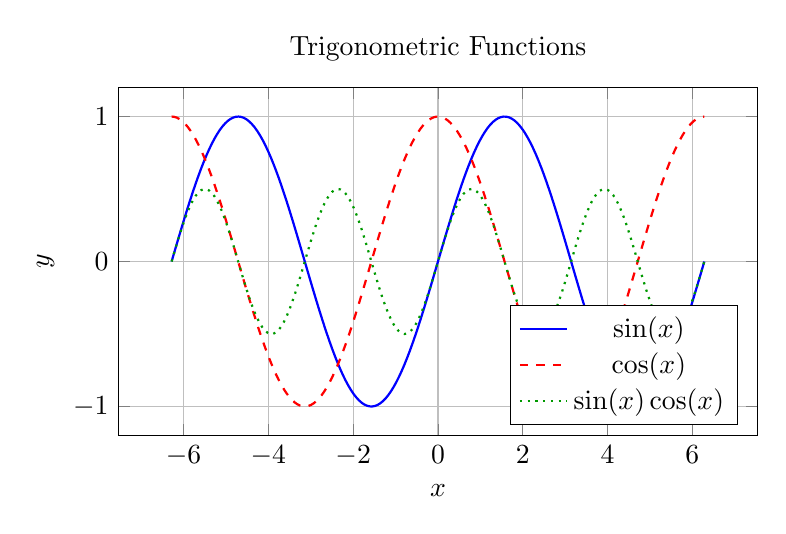
\begin{tikzpicture}
\begin{axis}[
  width=0.8\textwidth,
  height=6cm,
  xlabel={$x$},
  ylabel={$y$},
  title={Trigonometric Functions},
  legend pos=south east,
  grid=major,
  domain=-2*pi:2*pi,
  samples=200,
]
  \addplot[blue, thick] {sin(deg(x))};
  \addplot[red, thick, dashed] {cos(deg(x))};
  \addplot[green!60!black, thick, dotted] {sin(deg(x))*cos(deg(x))};
  \legend{$\sin(x)$, $\cos(x)$, $\sin(x)\cos(x)$}
\end{axis}
\end{tikzpicture}
\caption{Trigonometric functions and their product.}
\label{fig:trig}
\end{figure}

\begin{figure}[h!]
\centering
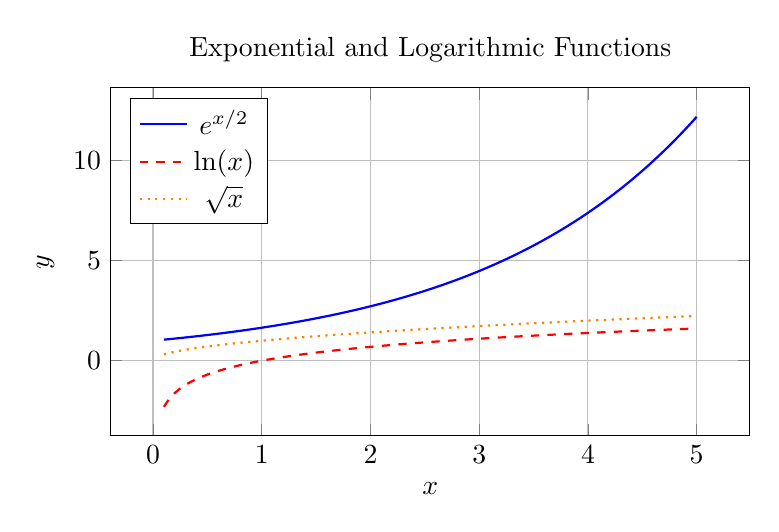
\begin{tikzpicture}
\begin{axis}[
  width=0.8\textwidth,
  height=6cm,
  xlabel={$x$},
  ylabel={$y$},
  title={Exponential and Logarithmic Functions},
  legend pos=north west,
  grid=major,
  domain=0.1:5,
  samples=100,
]
  \addplot[blue, thick] {exp(x/2)};
  \addplot[red, thick, dashed] {ln(x)};
  \addplot[orange, thick, dotted] {sqrt(x)};
  \legend{$e^{x/2}$, $\ln(x)$, $\sqrt{x}$}
\end{axis}
\end{tikzpicture}
\caption{Exponential, logarithmic, and square root functions.}
\label{fig:explog}
\end{figure}

\newpage

\subsection{Bar Charts}

\begin{figure}[h!]
\centering
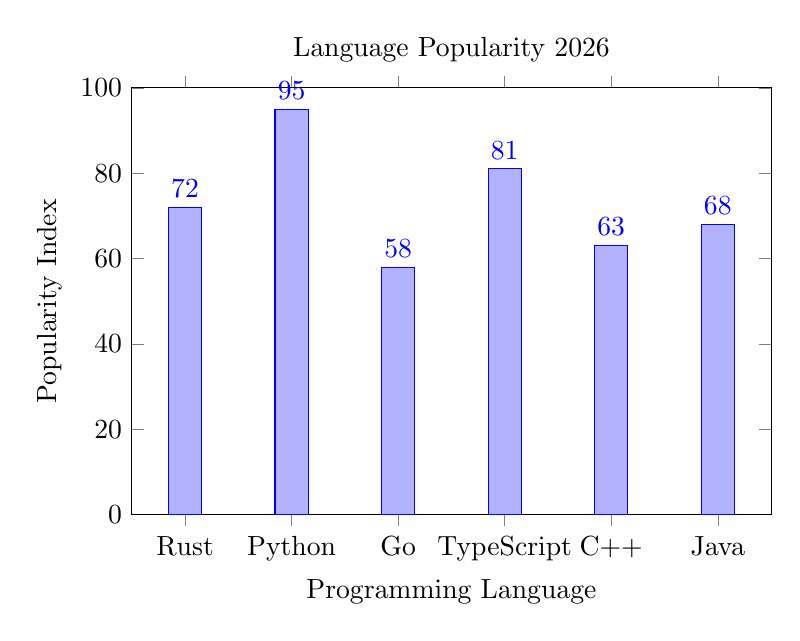
\begin{tikzpicture}
\begin{axis}[
  width=0.8\textwidth,
  height=7cm,
  ybar,
  bar width=12pt,
  xlabel={Programming Language},
  ylabel={Popularity Index},
  title={Language Popularity 2026},
  symbolic x coords={Rust, Python, Go, TypeScript, C++, Java},
  xtick=data,
  nodes near coords,
  nodes near coords align={vertical},
  ymin=0,
  ymax=100,
]
  \addplot coordinates {(Rust,72) (Python,95) (Go,58) (TypeScript,81) (C++,63) (Java,68)};
\end{axis}
\end{tikzpicture}
\caption{Programming language popularity indices (hypothetical data).}
\label{fig:barchart}
\end{figure}

\subsection{Scatter Plot with Regression}

\begin{figure}[h!]
\centering
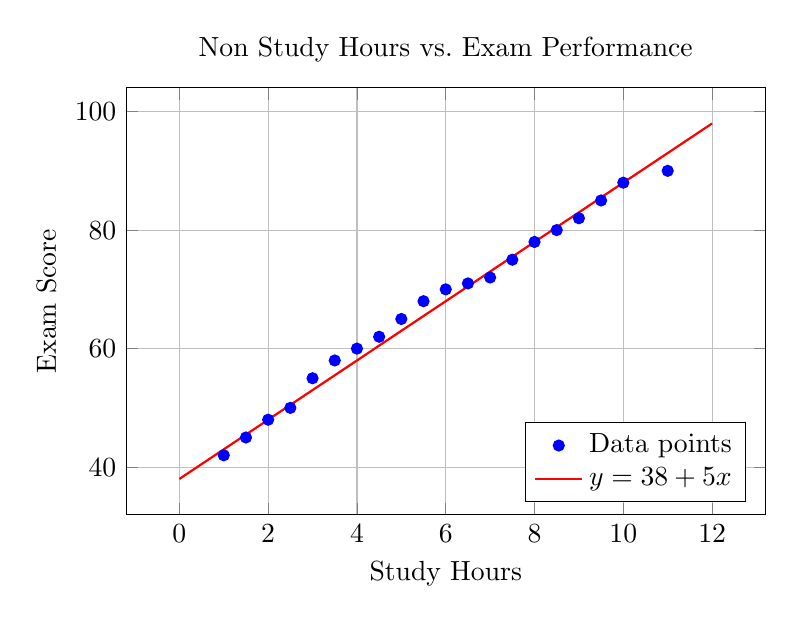
\begin{tikzpicture}
\begin{axis}[
  width=0.8\textwidth,
  height=7cm,
  xlabel={Study Hours},
  ylabel={Exam Score},
  title={Non Study Hours vs.\ Exam Performance},
  grid=major,
  legend pos=south east,
]
  \addplot[only marks, mark=*, blue] coordinates {
    (1,42) (2,48) (3,55) (4,60) (5,65) (6,70) (7,72) (8,78) (9,82)
    (10,88) (2.5,50) (3.5,58) (5.5,68) (7.5,75) (9.5,85) (4.5,62)
    (6.5,71) (8.5,80) (1.5,45) (11,90)
  };
  \addplot[red, thick, domain=0:12] {38 + 5*x};
  \legend{Data points, $y = 38 + 5x$}
\end{axis}
\end{tikzpicture}
\caption{Scatter plot with linear regression line.}
\label{fig:scatter}
\end{figure}

\newpage

\subsection{TikZ Diagrams}

\begin{figure}[h!]
\centering
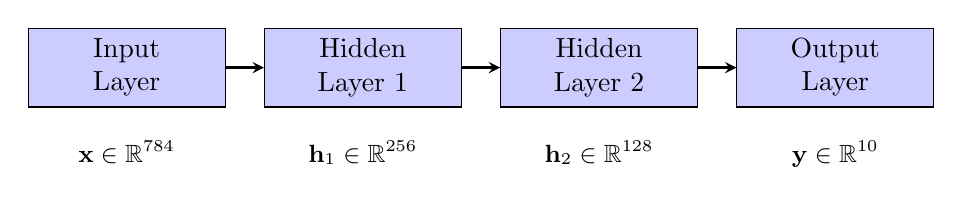
\begin{tikzpicture}[
  node distance=2cm,
  box/.style={rectangle, draw, fill=blue!20, minimum width=2.5cm, minimum height=1cm, align=center},
  arrow/.style={->, thick, >=stealth},
]
  \node[box] (input) {Input\\Layer};
  \node[box, right of=input, xshift=1cm] (hidden1) {Hidden\\Layer 1};
  \node[box, right of=hidden1, xshift=1cm] (hidden2) {Hidden\\Layer 2};
  \node[box, right of=hidden2, xshift=1cm] (output) {Output\\Layer};

  \draw[arrow] (input) -- (hidden1);
  \draw[arrow] (hidden1) -- (hidden2);
  \draw[arrow] (hidden2) -- (output);

  \node[below=0.3cm of input] {\small $\mathbf{x} \in \mathbb{R}^{784}$};
  \node[below=0.3cm of hidden1] {\small $\mathbf{h}_1 \in \mathbb{R}^{256}$};
  \node[below=0.3cm of hidden2] {\small $\mathbf{h}_2 \in \mathbb{R}^{128}$};
  \node[below=0.3cm of output] {\small $\mathbf{y} \in \mathbb{R}^{10}$};
\end{tikzpicture}
\caption{Architecture of a feedforward neural network.}
\label{fig:nn}
\end{figure}

\begin{figure}[h!]
\centering
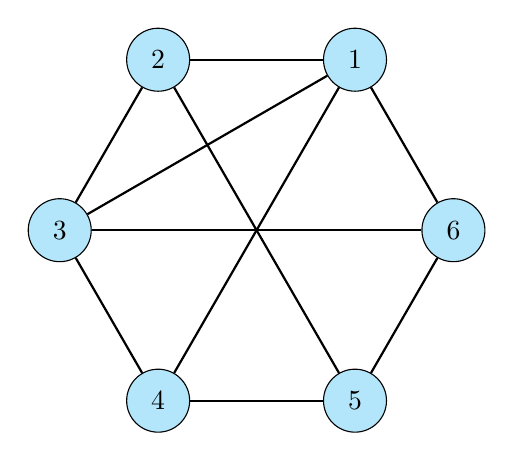
\begin{tikzpicture}
  % Nodes
  \foreach \i in {1,...,6} {
    \node[circle, draw, fill=cyan!30, minimum size=0.8cm] (n\i) at ({60*\i}:2.5cm) {\i};
  }
  % Edges
  \draw[thick] (n1) -- (n2);
  \draw[thick] (n2) -- (n3);
  \draw[thick] (n3) -- (n4);
  \draw[thick] (n4) -- (n5);
  \draw[thick] (n5) -- (n6);
  \draw[thick] (n6) -- (n1);
  \draw[thick] (n1) -- (n3);
  \draw[thick] (n1) -- (n4);
  \draw[thick] (n2) -- (n5);
  \draw[thick] (n3) -- (n6);
\end{tikzpicture}
\caption{A graph with 1 vertices and 10 edges.}
\label{fig:graph}
\end{figure}

\newpage

\subsection{Pie Chart sss}

\begin{figure}[h!]
\centering
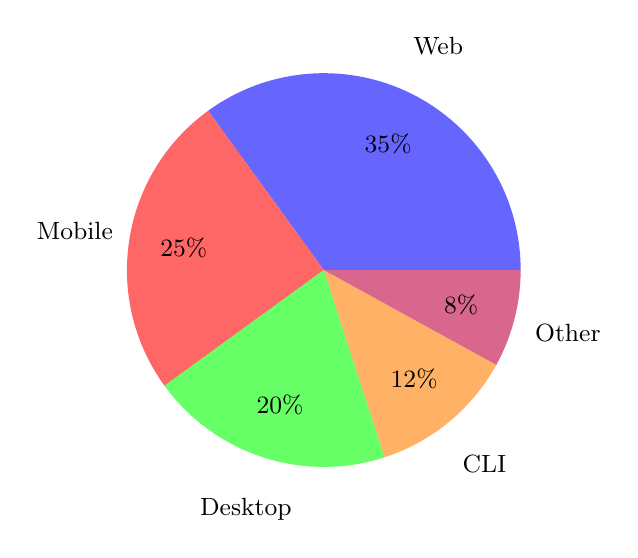
\begin{tikzpicture}
  % Web: 35%
  \fill[blue!60] (0,0) -- (0:2.5cm) arc (0:126:2.5cm) -- cycle;
  \node at (63:1.8cm) {\small 35\%};
  \node at (63:3.2cm) {\small Web};
  % Mobile: 25%
  \fill[red!60] (0,0) -- (126:2.5cm) arc (126:216:2.5cm) -- cycle;
  \node at (171:1.8cm) {\small 25\%};
  \node at (171:3.2cm) {\small Mobile};
  % Desktop: 20%
  \fill[green!60] (0,0) -- (216:2.5cm) arc (216:288:2.5cm) -- cycle;
  \node at (252:1.8cm) {\small 20\%};
  \node at (252:3.2cm) {\small Desktop};
  % CLI: 12%
  \fill[orange!60] (0,0) -- (288:2.5cm) arc (288:331.2:2.5cm) -- cycle;
  \node at (309.6:1.8cm) {\small 12\%};
  \node at (309.6:3.2cm) {\small CLI};
  % Other: 8%
  \fill[purple!60] (0,0) -- (331.2:2.5cm) arc (331.2:360:2.5cm) -- cycle;
  \node at (345.6:1.8cm) {\small 8\%};
  \node at (345.6:3.2cm) {\small Other};
\end{tikzpicture}
\caption{Software platform distribution (hypothetical).}
\label{fig:pie}
\end{figure}

\lipsum[8-9]

\newpage

% ============================================================================
% SECTION 6: Code Listings
% ============================================================================
\section{Source Code Listings}
\label{sec:code}

\subsection{Rust Implementation}

\begin{lstlisting}[language=C, caption={Binary search in Rust}, label=lst:binsearch]
fn binary_search(arr: &[i32], target: i32) -> Option<usize> {
    let mut low = 0;
    let mut high = arr.len();

    while low < high {
        let mid = low + (high - low) / 2;
        match arr[mid].cmp(&target) {
            Ordering::Less => low = mid + 1,
            Ordering::Greater => high = mid,
            Ordering::Equal => return Some(mid),
        }
    }
    None
}
\end{lstlisting}

\subsection{Python Data Processing}

\begin{lstlisting}[language=Python, caption={DataFrame operations in Python}, label=lst:pandas]
import pandas as pd
import numpy as np

def process_data(filepath: str) -> pd.DataFrame:
    """Load, clean, and transform a dataset."""
    df = pd.read_csv(filepath)

    # Remove duplicates and null values
    df = df.drop_duplicates()
    df = df.dropna(subset=['value', 'category'])

    # Feature engineering
    df['log_value'] = np.log1p(df['value'])
    df['zscore'] = (df['value'] - df['value'].mean()) / df['value'].std()

    # Aggregate by category
    summary = df.groupby('category').agg(
        mean_value=('value', 'mean'),
        std_value=('value', 'std'),
        count=('value', 'count'),
    ).reset_index()

    return summary
\end{lstlisting}

\subsection{SQL Query Example}

\begin{lstlisting}[language=SQL, caption={Complex SQL query with window functions}, label=lst:sql]
WITH monthly_revenue AS (
    SELECT
        DATE_TRUNC('month', order_date) AS month,
        product_category,
        SUM(amount) AS revenue
    FROM orders
    WHERE order_date >= '2025-01-01'
    GROUP BY 1, 2
)
SELECT
    month,
    product_category,
    revenue,
    LAG(revenue) OVER (
        PARTITION BY product_category
        ORDER BY month
    ) AS prev_month_revenue,
    revenue - LAG(revenue) OVER (
        PARTITION BY product_category
        ORDER BY month
    ) AS month_over_month_change
FROM monthly_revenue
ORDER BY product_category, month;
\end{lstlisting}

\lipsum[10]

\newpage

% ============================================================================
% SECTION 7: Tables
% ============================================================================
\section{Complex Table Layouts}
\label{sec:tables}

\subsection{Performance Comparison}

\begin{table}[h!]
\centering
\caption{Rendering performance across terminal emulators.}
\label{tab:perf}
\begin{tabular}{@{} l r r r r @{}}
\toprule
Terminal & FPS & Memory (MB) & Startup (ms) & Protocol \\
\midrule
Kitty         & 60  & 128  & 45   & Poopy Graphics \\
Ghostty       & 60  & 95   & 32   & Kitty Graphics \\
WezTerm       & 55  & 145  & 68   & iTerm2 \\
iTerm2        & 48  & 180  & 120  & iTerm2 \\
Alacritty     & 30  & 42   & 15   & Sixel \\
Terminal.app  & 24  & 200  & 250  & Halfblocks \\
\bottomrule
\end{tabular}
\end{table}

\subsection{Algorithm Complexity}

\begin{table}[h!]
\centering
\caption{Time complexity of common sorting algorithms.}
\label{tab:sorting}
\begin{tabular}{@{} l c c c l @{}}
\toprule
Algorithm & Best & Average & Worst & Stable? \\
\midrule
Bubble Sort    & $O(n)$          & $O(n^2)$        & $O(n^2)$        & Yes \\
Selection Sort & $O(n^2)$        & $O(n^2)$        & $O(n^2)$        & No \\
Insertion Sort & $O(n)$          & $O(n^2)$        & $O(n^2)$        & Yes \\
Merge Sort     & $O(n \log n)$   & $O(n \log n)$   & $O(n \log n)$   & Yes \\
Quick Sort     & $O(n \log n)$   & $O(n \log n)$   & $O(n^2)$        & No \\
Heap Sort      & $O(n \log n)$   & $O(n \log n)$   & $O(n \log n)$   & No \\
Tim Sort       & $O(n)$          & $O(n \log n)$   & $O(n \log n)$   & Yes \\
Radix Sort     & $O(nk)$         & $O(nk)$         & $O(nk)$         & Yes \\
\bottomrule
\end{tabular}
\end{table}

\subsection{Not so Wide Table with TabularX}

\begin{table}[h!]
\centering
\caption{Feature comparison across document formats.}
\label{tab:formats}
\begin{tabularx}{\textwidth}{@{} l X X X @{}}
\toprule
Feature & PDF & EPUB & DjVu \\
\midrule
Text reflow & No, fixed layout & Yes, reflowable & No, fixed layout \\
Image support & Full (vector + raster) & Raster only (PNG, JPEG, WebP) & Compressed raster \\
Math rendering & Native (via LaTeX) & MathML or images & Not supported \\
File size & Medium to large & Small to medium & Very small \\
Annotations & Rich (PDF standard) & Limited & Not supported \\
Accessibility & Improving (tagged PDF) & Good (HTML) & Poor \\
\bottomrule
\end{tabularx}
\end{table}

\lipsum[11-12]

\newpage

% ============================================================================
% SECTION 8: Mixed Content Pages
% ============================================================================
\section{Mixed Content}
\label{sec:mixed}

section deliberately mixes content types on the same page to test SyncTeX
coordinate mapping across heterogeneous layouts.

\subsection{Text Interleaved with Math}

Consider the optimization problem of minimizing $f(x) = x^2 + 2x + 1$. Taking
the derivative and setting it to zero: $f'(x) = 2x + 2 = 0$, which gives
$x = -1$. Since $f''(x) = 2 > 0$, this is indeed a minimum. The minimum value
is $f(-1) = (-1)^2 + 2(-1) + 1 = 0$.

More generally, for a quadratic $f(x) = ax^2 + bx + c$ with $a > 0$, the
minimum occurs at:
\begin{equation}
  x^* = -\frac{b}{2a}, \qquad f(x^*) = c - \frac{b^2}{4a}
\end{equation}

Not now consider the multivariate case. Given $f(\mathbf{x}) = \mathbf{x}^T A \mathbf{x} + \mathbf{b}^T \mathbf{x} + c$
where $A$ is positive definite, the gradient is:
\begin{equation}
  \nabla f = 2A\mathbf{x} + \mathbf{b}
\end{equation}
and the minimum is at $\mathbf{x}^* = -\frac{1}{2}A^{-1}\mathbf{b}$.

\subsection{Inline Diagram with Discussion}

Figure~\ref{fig:workflow} shows a typical data processing workflow. Raw data
enters from the left, passes through validation and transformation stages,
and produces clean output on the right.

\begin{figure}[h!]
\centering
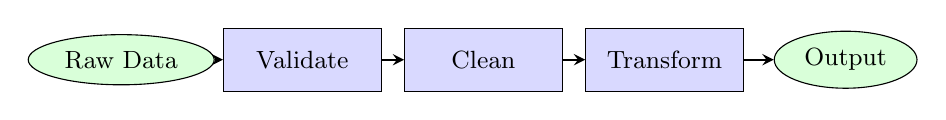
\begin{tikzpicture}[
  node distance=1.5cm,
  stage/.style={rectangle, draw, fill=blue!15, minimum width=2cm, minimum height=0.8cm, font=\small},
  data/.style={ellipse, draw, fill=green!15, minimum width=1.5cm, font=\small},
  arrow/.style={->, thick, >=stealth},
]
  \node[data] (raw) {Raw Data};
  \node[stage, right of=raw, xshift=0.8cm] (validate) {Validate};
  \node[stage, right of=validate, xshift=0.8cm] (clean) {Clean};
  \node[stage, right of=clean, xshift=0.8cm] (transform) {Transform};
  \node[data, right of=transform, xshift=0.8cm] (output) {Output};

  \draw[arrow] (raw) -- (validate);
  \draw[arrow] (validate) -- (clean);
  \draw[arrow] (clean) -- (transform);
  \draw[arrow] (transform) -- (output);
\end{tikzpicture}
\caption{Data processing workflow.}
\label{fig:workflow}
\end{figure}

After transformation, the data can be analyzed using the methods described
in Section~\ref{sec:stats}. The resulting statistics are summarized in
Table~\ref{tab:summary}.

\begin{table}[h!]
\centering
\caption{Summary statistics after data processing.}
\label{tab:summary}
\begin{tabular}{@{} l r r r r @{}}
\toprule
Variable & Mean & Std Dev & Min & Max \\
\midrule
Temperature ($^\circ$C) & 22.4 & 5.1 & 8.2 & 38.7 \\
Humidity (\%) & 65.3 & 12.8 & 25.0 & 95.0 \\
Pressure (hPa) & 1013.2 & 8.4 & 985.1 & 1035.6 \\
Wind Speed (m/s) & 4.7 & 2.3 & 0.1 & 15.8 \\
\bottomrule
\end{tabular}
\end{table}

\subsection{Code with Mathematical Explanation}

The following Rust code implements gradient descent. The update rule is:
\begin{equation}
  \mathbf{x}_{t+1} = \mathbf{x}_t - \alpha \nabla f(\mathbf{x}_t)
\end{equation}
where $\alpha$ is the learning rate.

\begin{lstlisting}[language=C, caption={Gradient descent implementation}]
fn gradient_descent(
    f: impl Fn(f64) -> f64,
    df: impl Fn(f64) -> f64,
    x0: f64,
    lr: f64,
    iterations: usize,
) -> f64 {
    let mut x = x0;
    for _ in 0..iterations {
        x -= lr * df(x);
    }
    x
}
\end{lstlisting}

\lipsum[13-14]

\newpage

% ============================================================================
% SECTION 9: Extended Prose
% ============================================================================
\section{Extended Prose Passages}
\label{sec:prose}

\subsection{On the Nature of Computation}

The history of computation stretches back thousands of years, from the abacus
to the modern microprocessor. At its core, computation is about transforming
information according to well-defined rules. The ancient Greeks developed
algorithms for computing greatest common divisors, while Babylonian
mathematicians had methods for approximating square roots.

In the seventeenth century, Leibniz and Pascal built mechanical calculators
capable of performing arithmetic operations. These devices, while limited,
demonstrated that mathematical reasoning could be mechanized. Leibniz went
further, dreaming of a universal calculus that could resolve all disputes
through computation --- a vision that would take three centuries to fully
appreciate.

Charles Babbage's Analytical Engine, designed in the 1830s, represented a
conceptual leap: a general-purpose computing machine with memory, a processor,
and the ability to be programmed using punched cards. Ada Lovelace, working
with Babbage, wrote what is considered the first computer program and foresaw
that the engine could manipulate symbols beyond mere numbers.

The twentieth century brought the formalization of computation. In 1936,
Alan Turing published his landmark paper introducing the Turing machine,
an abstract device that captures the essence of algorithmic computation.
Simultaneously, Alonzo Church developed the lambda calculus, providing an
equivalent but syntactically different foundation. The Church-Turing thesis
asserts that any effectively computable function can be computed by a
Turing machine.

\subsection{The Rise of Programming Languages}

The first electronic computers were programmed in machine code --- sequences
of binary instructions specific to each hardware architecture. This was
tedious and error-prone. The development of assembly language provided
human-readable mnemonics, but programs remained tied to specific machines.

Fortran, developed by John Backus at IBM in the 1950s, was the first
high-level programming language to gain widespread adoption. It allowed
scientists and engineers to express computations in mathematical notation
rather than machine instructions. The Fortran compiler translated these
high-level expressions into efficient machine code.

LISP, created by John McCarthy in 1958, took a radically different approach.
Based on Church's lambda calculus, LISP treated code and data uniformly as
list structures. This homoiconicity enabled powerful metaprogramming
capabilities and made LISP the language of choice for artificial intelligence
research for decades.

The 1970s saw the development of C by Dennis Ritchie at Bell Labs. C provided
low-level access to memory while maintaining enough abstraction to write
portable programs. Unix, rewritten in C, demonstrated that an entire operating
system could be implemented in a high-level language. The combination of C
and Unix would shape computing for the next fifty years.

\subsection{Types, Safety, and Correctness}

As software systems grew in complexity, the cost of bugs became increasingly
apparent. The Ariane 5 rocket explosion in 1996, caused by an integer overflow
in a type conversion, destroyed a payload worth \$370 million. The Therac-25
radiation therapy machine killed patients due to race conditions in its
control software. These disasters motivated research into programming
language safety.

Type systems provide a lightweight form of verification. A type system
assigns types to expressions and checks that operations are applied to
compatible types. Static type systems, like those in Haskell, Rust, and
Standard ML, catch type errors at compile time. Dynamic type systems, like
those in Python and JavaScript, defer type checking to runtime.

Rust, developed at Mozilla and first released in 2010, introduced the concept
of ownership and borrowing to prevent memory safety bugs without garbage
collection. The borrow checker enforces at compile time that references
cannot outlive the data they point to, and that mutable references are
exclusive. This eliminates entire categories of bugs: use-after-free,
double-free, data races, and null pointer dereferences.

The formal verification community has developed tools that go beyond type
checking. Proof assistants like Coq, Lean, and Agda allow programmers to
write mathematical proofs that their code satisfies its specification.
The CompCert C compiler, verified in Coq, guarantees that the compiled
code preserves the semantics of the source program.

\subsection{Distributed Systems and Consensus}

Modern computing is inherently distributed. Cloud services run across
thousands of machines in data centers spanning continents. Mobile
applications communicate with backend servers over unreliable networks.
The challenge of distributed systems is achieving consistency and
availability despite partial failures.

The CAP theorem, proved by Eric Brewer in 2000, states that a distributed
system cannot simultaneously guarantee consistency (all nodes see the same
data), availability (every request receives a response), and partition
tolerance (the system continues operating despite network partitions).
Since network partitions are inevitable in practice, system designers must
choose between consistency and availability.

Consensus algorithms allow a group of processes to agree on a value despite
failures. Paxos, developed by Leslie Lamport in 1989, was the first
practical consensus algorithm. Its correctness proof is elegant but the
algorithm is notoriously difficult to implement. Raft, designed by Diego
Ongaro and John Ousterhout in 2014, achieves the same guarantees with a
more understandable decomposition into leader election, log replication,
and safety.

Blockchain technology, introduced by Satoshi Nakamoto in 2008, solves
consensus in an open network where participants may be adversarial.
Bitcoin's proof-of-work mechanism requires miners to solve computational
puzzles, making it expensive to tamper with the transaction history.
Ethereum extended this model to support arbitrary computation through
smart contracts.

\subsection{The Future of Computing}

Quantum computing promises exponential speedups for certain problems.
Shor's algorithm can factor large integers in polynomial time, threatening
current cryptographic systems. Grover's algorithm provides a quadratic
speedup for unstructured search. However, building reliable quantum
computers remains an enormous engineering challenge due to decoherence
and error rates.

Neuromorphic computing takes inspiration from biological neural networks.
Instead of the von Neumann architecture's separation of memory and
processing, neuromorphic chips integrate computation and storage in
networks of artificial neurons. Intel's Loihi chip and IBM's TrueNorth
represent early examples of this paradigm.

The convergence of these trends --- powerful type systems, formal
verification, distributed consensus, quantum computing, and neuromorphic
architectures --- suggests that the future of computing will be
fundamentally different from its past. The software that runs on these
new platforms will need new abstractions, new programming models, and
new ways of reasoning about correctness.

% ============================================================================
% SECTION 10: Appendix with Dense Formulas
% ============================================================================
\newpage
\appendix
\section{Mathematical Reference}

\subsection{Fourier Transform}
\begin{equation}
  \hat{f}(\xi) = \int_{-\infty}^{\infty} f(x) e^{-2\pi i x \xi}\,dx
\end{equation}

\subsection{Laplace Transform}
\begin{equation}
  F(s) = \mathcal{L}\{f(t)\} = \int_0^{\infty} f(t) e^{-st}\,dt
\end{equation}

\subsection{Euler's Identity}
\begin{equation}
  e^{i\pi} + 1 = 0
\end{equation}

\subsection{Navier--Stokes Equations}
\begin{equation}
  \rho\left(\frac{\partial \mathbf{u}}{\partial t} + \mathbf{u} \cdot \nabla \mathbf{u}\right)
  = -\nabla p + \mu \nabla^2 \mathbf{u} + \mathbf{f}
\end{equation}

\subsection{Maxwell's Equations}
\begin{align}
  \nabla \cdot \mathbf{E} &= \frac{\rho}{\varepsilon_0} \\
  \nabla \cdot \mathbf{B} &= 0 \\
  \nabla \times \mathbf{E} &= -\frac{\partial \mathbf{B}}{\partial t} \\
  \nabla \times \mathbf{B} &= \mu_0 \mathbf{J} + \mu_0 \varepsilon_0 \frac{\partial \mathbf{E}}{\partial t}
\end{align}

\subsection{Schrodinger Equation}
\begin{equation}
  i\hbar \frac{\partial}{\partial t} \Psi(\mathbf{r}, t)
  = \left[-\frac{\hbar^2}{2m}\nabla^2 + V(\mathbf{r}, t)\right]\Psi(\mathbf{r}, t)
\end{equation}

\subsection{General Relativity}
\begin{equation}
  R_{\mu\nu} - \frac{1}{2}Rg_{\mu\nu} + \Lambda g_{\mu\nu} = \frac{8\pi G}{c^4}T_{\mu\nu}
\end{equation}

\subsection{Stokes' Theorem}
\begin{equation}
  \oint_{\partial \Omega} \omega = \int_{\Omega} d\omega
\end{equation}

\subsection{Cauchy's Integral Formula}
\begin{equation}
  f(a) = \frac{1}{2\pi i} \oint_\gamma \frac{f(z)}{z - a}\,dz
\end{equation}

\subsection{Riemann Zeta Function}
\begin{equation}
  \zeta(s) = \sum_{n=1}^{\infty} \frac{1}{n^s} = \prod_{p \text{ prime}} \frac{1}{1 - p^{-s}}, \quad \Re(s) > 1
\end{equation}

\end{document}
